% =========================================================================
%  Treatment Limitation Documentation and Risk Adjusted Mortality
%  Benchmarking in 190 US Intensive Care Units
%
%  Target: Annals of the American Thoracic Society
%  Compile: pdflatex Manuscript.tex  (twice, for cross references)
%  Serif throughout per author preference.
% =========================================================================
\documentclass[12pt,a4paper]{article}

\usepackage[margin=1in]{geometry}
\usepackage{newtxtext,newtxmath}     % Times based serif, text and maths
\usepackage{setspace}
\usepackage{lineno}
\usepackage{graphicx}
\usepackage{booktabs}
\usepackage{siunitx}
\usepackage{caption}
\usepackage{array}
\usepackage{longtable}
\usepackage[hidelinks]{hyperref}
\usepackage{authblk}

\doublespacing
\linenumbers
\captionsetup{font=small,labelfont=bf,justification=raggedright,
              singlelinecheck=false}
\setlength{\parskip}{0pt}
\setlength{\parindent}{1.5em}
\renewcommand{\arraystretch}{1.15}

\title{\textbf{Treatment Limitation Documentation and Risk Adjusted Mortality
Benchmarking in 190 US Intensive Care Units}}

\author[1]{Author One}
\author[1]{Author Two}
\affil[1]{Affiliation to be completed}
\date{}

\begin{document}
\maketitle

\noindent\textbf{Running head.} Treatment limitation and ICU benchmarking\\
\textbf{Word count, body.} 2704\\
\textbf{Tables.} 3 \quad \textbf{Figures.} 3 \quad \textbf{Supplementary.} separate file\\
\textbf{Keywords.} intensive care, benchmarking, standardized mortality ratio,
treatment limitation, code status, risk adjustment

\newpage
% =========================================================================
\section*{Abstract}
\begin{spacing}{1.15}
\noindent\textbf{Rationale.} Standardized mortality ratios derived from severity
of illness scores are used to compare intensive care unit performance. These
scores estimate the probability of death under full treatment and contain no
term for treatment limitation. Units differ in how often such limitations are
documented.

\noindent\textbf{Objective.} To determine whether between unit variation in
treatment limitation documentation reflects patient case mix or local practice,
and to quantify its consequences for risk adjusted mortality benchmarking.

\noindent\textbf{Methods.} Retrospective analysis of 136{,}236 adult admissions
to 190 US intensive care units in the eICU Collaborative Research Database
during 2014 and 2015. Treatment limitation documented within 24 hours of
admission was classified on an ordered scale from full therapy to comfort
measures only. We assessed APACHE IVa calibration within limitation strata. We
compared patient characteristics between units in the highest and lowest
quintile of limitation rate before and after inverse probability weighting. We
then ranked units by standardized mortality ratio with and without limitation
status in the risk model.

\noindent\textbf{Measurements and Main Results.} Code status was documented in
96.1\% of admissions. A limitation beyond full therapy was present in 9.9\%. The
APACHE IVa calibration slope was 1.005 with an intercept of $-0.425$. The
standardized mortality ratio rose from 0.62 under full therapy to 1.87 under
comfort measures only. The integrated calibration index was 0.342 in the comfort
measures stratum and 0.037 to 0.057 elsewhere. After weighting until all 13
measured covariates balanced, units in the highest limitation quintile still
documented limitation 2.89 times as often as units in the lowest quintile,
compared with 3.58 times before weighting. Adding limitation status to the risk
model changed quartile assignment for 23.5\% of units and reversed mortality
outlier classification for 8.0\%. The direction of movement was predicted by a
unit's limitation rate with a Spearman correlation of $-0.689$. Excluding the 878
admissions under comfort measures orders, six in every thousand, reclassified
11.1\% of units.

\noindent\textbf{Conclusions.} Units differ severalfold in how often treatment
limitation is documented and patient case mix does not account for it. Risk
adjusted mortality benchmarking that ignores these decisions systematically
disadvantages units that document limitations more often.
\end{spacing}

\newpage
% =========================================================================
\section*{1. Introduction}

End of life practice varies widely between intensive care units. Withdrawal of
life sustaining treatment among patients who die ranges from 0 to 84\% across
published cohorts \cite{ref1}. The Ethicus-2 investigators found comparable
variation across 199 units in 36 countries \cite{ref2}. Variation has been
documented between countries, between regions and between units within a single
country \cite{ref1,ref3,ref4}. Two academic centers at opposite extremes of
treatment intensity differed in decision making norms rather than in patients
\cite{ref5}. Hospital level measures of end of life treatment intensity have
been developed and validated for precisely this reason \cite{ref6}. Hart and
colleagues studied 277{,}693 admissions to 141 US units and found the proportion
admitted with existing treatment limitations ranged from under 1\% to 20.9\%
after risk adjustment \cite{ref7}. Measurable center characteristics did not
explain that variation \cite{ref7}.

Treatment limitation is common in critical illness. Do not resuscitate orders
were recorded in 13\% of 24{,}790 admissions to one tertiary unit over 19 years
\cite{ref8}, and in 36.6\% of a medical intensive care cohort when orders for
life sustaining treatment were included \cite{ref9}. Timing varies, with roughly
a quarter of orders written within 48 hours of admission and the remainder later
\cite{ref10}. These orders carry substantial prognostic weight. Mortality among
patients with such orders is several times that of patients without them
\cite{ref9,ref11}, and the association persists after propensity matching
\cite{ref12}. Placing an order also changes subsequent care, including the
intensity of interventions delivered \cite{ref13}.

Severity of illness scores estimate the probability of death under full
treatment. The APACHE method was introduced in 1985 and validated on 5815 admissions
from 13 hospitals \cite{ref14}. The APACHE IVa model was derived from 110{,}558
admissions to 104 units during 2002 and 2003 \cite{ref15}. Its covariates describe physiology, age, comorbidity and admission
diagnosis \cite{ref15}. Comparable models including SAPS 3 share this structure
\cite{ref16,ref17}. No covariate in any of them represents a decision to withhold
resuscitation. An order not to resuscitate alters the probability of death
without altering any variable the model observes.

The performance of these models is known to be unstable. Discrimination and
calibration deteriorate as practice changes, which is why successive versions
have been required \cite{ref18,ref19}. Performance also differs across ethnic groups within the same health
system \cite{ref20}. Calibration is generally the first property to fail while
discrimination is preserved \cite{ref18}.

Standardized mortality ratios derived from these scores are the accepted currency
of intensive care benchmarking \cite{ref21}. Units are compared and ranked on
observed deaths divided by predicted deaths, and in some systems reimbursed on
that basis \cite{ref21}. The ratio is assumed to isolate quality of care
once case mix is accounted for \cite{ref21}. Several lines of evidence suggest
the assumption is fragile. Glance and colleagues showed that the choice of
scoring system determines which units are labeled outliers \cite{ref21}. Kramer
and colleagues compared APACHE IVa against a National Quality Forum model across
89{,}353 admissions and found the two agreed on the direction and significance of
the standardized mortality ratio in only 45\% of units \cite{ref22}. Admission
patterns alone alter mortality based performance measures \cite{ref23}. Risk
adjusted mortality carries conceptual limits that constrain its use as a quality
signal, since a statistically unexpected death is not the same as a preventable
one \cite{ref24}. Model misspecification introduces bias into the resulting
quality measures \cite{ref25}, and alternative modeling strategies produce
materially different unit level estimates \cite{ref26,ref27}.

Whether treatment limitation practice distorts these comparisons has not been
tested. Hart and colleagues proposed that advance care planning norms contribute
to variation in intensive care use and demonstrated the mechanism by simulation
\cite{ref28}. Feng and Dubin identified variables associated with incorrect
APACHE IVa predictions in a multicenter database and included the frequency of
care limitation change among them, but examined classification error rather than
calibration \cite{ref29}. No study has measured the consequence for risk adjusted
mortality benchmarking in observed data.

We examined 136{,}236 admissions to 190 US intensive care units. We asked whether
APACHE IVa calibration depends on documented treatment limitation, whether
between unit variation in limitation survives balancing of patient case mix, and
whether accounting for limitation changes how units are ranked.

% =========================================================================
\section*{2. Methods}

\subsection*{Data source}
We analyzed the eICU Collaborative Research Database version 2.0, which contains
200{,}859 unit stays at 208 US hospitals participating in a tele critical care
program during 2014 and 2015 \cite{ref30}. The database carries vital signs,
laboratory values, care plan documentation, severity scores and outcomes
\cite{ref30}, and has been characterized in detail elsewhere \cite{ref31}. It is
deidentified and was accessed under a data use agreement following completion of
human subjects research training \cite{ref30}. Institutional review board
approval was waived for analysis of this deidentified resource. Reporting follows
the TRIPOD recommendations for studies evaluating prediction models
\cite{ref32,ref33}.

\subsection*{Cohort}
Of 200{,}859 adult unit stays, 52{,}327 were excluded because no APACHE IVa result
was recorded and a further 12{,}296 because the predicted hospital mortality was
unavailable or zero, leaving 136{,}236 stays at 190 units. Unit level analyses were
restricted to the 162 units contributing 100 or more stays, excluding 911 stays in
28 smaller units and leaving 135{,}325 admissions. Figure~S1 shows the derivation.

\subsection*{Exposure}
Treatment limitation was taken from structured care plan documentation. For each
stay we recorded the most restrictive value documented within 24 hours of unit
admission on an ordered scale. Full therapy formed the reference. Limitation of
resuscitation type comprised do not resuscitate, no cardiopulmonary
resuscitation, no intubation and no cardioversion. Partial withdrawal comprised
no vasopressors or inotropes, no augmentation of care, no blood products and no
blood draws. Comfort measures only formed the most restrictive category. Stays
with no entry were retained as an undocumented category and reported but not
interpreted. The 24 hour window follows prior work distinguishing early from late
limitation orders \cite{ref10} and limits the degree to which the exposure
reflects deterioration occurring later in the stay.

\subsection*{Outcome}
In hospital mortality was compared against APACHE IVa predicted hospital
mortality.

\subsection*{Statistical analysis}
Calibration was assessed by logistic recalibration, regressing observed mortality
on the logit of predicted mortality. A slope of 1 and an intercept of 0 indicate
perfect calibration. Within strata we report the standardized mortality ratio and
the integrated calibration index, the mean absolute difference between a smoothed
observed risk and the predicted risk \cite{ref34,ref35}. Standard errors were
clustered on unit throughout.

The independent contribution of limitation status was estimated by adding it to a
recalibration model containing the APACHE linear predictor. Malignancy was
included to test whether an established source of miscalibration behaves
similarly \cite{ref36}. Discrimination was assessed on a random 30\% holdout of
40{,}871 admissions by area under the receiver operating characteristic curve
with DeLong's test and by Brier score.

To distinguish practice from case mix we compared units in the highest and lowest
quintile of limitation rate. Patient characteristics were balanced by inverse
probability of treatment weighting estimated by logistic regression, following
recommended practice \cite{ref37}. Balance was assessed by standardized mean
differences against a threshold of 0.1 \cite{ref37}. We then compared limitation
rates between quintiles before and after weighting. If case mix accounted for the
difference, balancing case mix should remove it. Between unit variation was
additionally summarized by the intraclass correlation coefficient and the median
odds ratio from mixed effects models with a unit random intercept
\cite{ref38,ref39}.

To quantify the benchmarking consequence, expected deaths per unit were computed
twice. The first used a recalibrated APACHE IVa model representing current
practice. The second added limitation status. Units were ranked by standardized
mortality ratio under each and compared on rank shift, quartile change and
outlier status using exact Poisson 95\% limits following Spiegelhalter
\cite{ref40}. We additionally evaluated two simpler strategies, excluding
admissions under comfort measures orders and excluding all admissions with any
limitation. Analyses used R version 4.6.0.

% =========================================================================
\section*{3. Results}

\subsection*{Cohort}
Among 136{,}236 admissions, mean APACHE IVa predicted mortality was 11.8\%
against observed mortality of 8.85\%, giving an overall standardized mortality
ratio of 0.75. Code status was documented within 24 hours in 96.1\% of
admissions. A limitation beyond full therapy was present in 13{,}496 admissions,
or 9.9\%. Table~\ref{tab:cohort} shows cohort characteristics by limitation
status. Patients with any limitation were older, with a median age of 77 years in
the resuscitation limitation group against 63 years under full therapy. They were
more severely ill, with a median APACHE IVa score of 66 against 49. Patients
under comfort measures orders had a median APACHE IVa score of 85 and a median
unit stay of 18.2 hours.

\subsection*{APACHE IVa calibration depends on treatment limitation}
The overall calibration slope was 1.005 with an intercept of $-0.425$. The model
ranks patients almost perfectly and is uniformly displaced, over predicting death
across the entire risk range. This pattern of preserved discrimination with
failed calibration matches that described for severity scores in contemporary
cohorts \cite{ref18}.

Calibration differed sharply by limitation status
(Figure~\ref{fig:performance}A, Table~\ref{tab:calibration}). The standardized
mortality ratio was 0.62 under full therapy, 1.17 with resuscitation limitation,
1.22 with partial withdrawal and 1.87 under comfort measures only. The integrated
calibration index was 0.039, 0.037 and 0.057 in the first three strata and 0.342
under comfort measures. In that stratum the model is not miscalibrated but
uninformative.

In a recalibration model with full therapy as reference, the adjusted odds of
death were 2.63 with resuscitation limitation, 2.97 with partial withdrawal and
15.30 under comfort measures only (Figure~\ref{fig:performance}B). Metastatic or
hematologic malignancy carried an adjusted odds ratio of 1.15. Adding limitation
status reduced model deviance by 3.6\% against 0.0\% for malignancy, and the
likelihood ratio statistic was 2136 against 17.

On held out data, adding limitation status improved the area under the curve from
0.8657 to 0.8760, significant by DeLong's test at $p<0.001$, and reduced the
Brier score from 0.0621 to 0.0579 (Table~S1). Adding malignancy
changed the area under the curve by 0.0001, which was not significant.

\subsection*{Variation between units is not explained by case mix}
Across 162 units, limitation rates ranged from 0 to 27.5\% with a median of
10.5\% (Figure~\ref{fig:variation}A). One unit documented no limitation across
more than 100 admissions.

Units in the highest limitation quintile differed from those in the lowest on two
of 13 measured characteristics before weighting. Patients were older, with a
standardized mean difference of 0.197, and more often admitted from the emergency
department, at 0.149. Severity was near identical, at $-0.006$ for the APACHE IVa
score and 0.008 for predicted mortality.

After inverse probability weighting all 13 covariates balanced within the 0.1
threshold (Figure~\ref{fig:variation}B). Age fell to $-0.004$ and admission from
the emergency department to 0.004. Despite complete balance on measured
characteristics, units in the highest quintile documented limitation in 16.5\% of
admissions against 5.7\% in the lowest, a ratio of 2.89. The unweighted ratio was
3.58. Approximately four fifths of the difference in practice survived balancing
of patient case mix.

Mixed effects models gave the same answer. The intraclass correlation was 0.084
before adjustment and 0.104 after adjustment for case mix. The median odds ratio
rose from 1.69 to 1.80, indicating that moving a patient between randomly chosen
units changes the odds of documented limitation by close to twofold
\cite{ref39}.

\subsection*{Consequences for benchmarking}
Adding limitation status to the risk model preserved the overall ordering of
units, with a Spearman correlation of 0.949, while moving individual units
substantially (Table~S2). The median absolute rank shift was 7.5
positions of 162. Sixty two units moved more than 10 positions and 24 moved more
than 20.

Thirty eight units, or 23.5\%, changed quartile. Thirteen units, or 8.0\%,
changed outlier classification against exact Poisson limits \cite{ref40}. Four
units previously flagged as high mortality became unremarkable and three
previously unremarkable units became outliers
(Figure~\ref{fig:benchmarking}B).

Movement was systematic. The signed rank shift correlated with a unit's
limitation rate at a Spearman coefficient of $-0.689$
(Figure~\ref{fig:benchmarking}A). Units in the lowest limitation quintile moved
from a standardized mortality ratio of 0.984 to 1.027. Units in the highest
quintile moved from 1.013 to 0.876. Under current benchmarking these quintiles
appear equivalent. After accounting for limitation they do not.

\subsection*{A simpler remedy}
Excluding the 878 admissions under comfort measures orders, 0.6\% of the cohort,
reclassified 18 units across quartiles, or 11.1\% (Table~\ref{tab:remedy}). Full
adjustment for the ordered limitation scale reclassified 38 units, or 23.5\%.
Excluding all 13{,}496 admissions with any limitation reclassified 46 units, or
28.4\%. Excluding the smallest group recovered roughly half the effect of full
adjustment.

% =========================================================================
\section*{4. Discussion}

APACHE IVa calibration depends on a decision the model does not observe. The
standardized mortality ratio was 0.62 among patients receiving full therapy and
1.87 among patients under comfort measures. The integrated calibration index in
that stratum was nine times larger than elsewhere \cite{ref34}. The model is not
merely displaced in these patients. It is uninformative.

Documentation of limitation varied severalfold between units and patient case mix
did not account for it. This extends Hart and colleagues, who reported comparable
variation after regression adjustment in a different database a decade earlier
\cite{ref7}. Our design equalized the covariate distributions rather than
adjusting for them \cite{ref37}, and roughly four fifths of the practice
difference persisted. Limitation rates were higher in our cohort than in theirs,
10.5\% against 4.0\%, consistent with the expansion of palliative care services
over the intervening period. Palliative care consultation more than doubles
transition to limitation orders in randomized comparison, from 23.4\% to 50.5\%
\cite{ref41}, and integration of palliative care into critical care alters both
process and outcome measures \cite{ref42,ref43}. Units therefore differ in
limitation rate partly because they differ in service configuration, which is a
property of the unit rather than of its patients \cite{ref5}.

The consequence for benchmarking is substantial. Accounting for limitation moved
23.5\% of units across quartiles and reversed outlier classification for 8.0\%.
Kramer and colleagues found that substituting an entirely different risk model
changed the direction and significance of the standardized mortality ratio in
55\% of units \cite{ref22}. Glance and colleagues reached a similar conclusion
comparing scoring systems \cite{ref21}, and admission patterns alone have been
shown to shift these measures \cite{ref23}. We find that a single variable
already recorded in 96\% of charts moves a quarter of quartile assignments. The
intervention is far smaller and the effect is of comparable order.

Whether to adjust for limitation status is a genuine question and we do not
resolve it. Adjustment treats limitation as patient preference and therefore as
case mix. Withholding adjustment treats it as modifiable unit behavior. Both
positions are defensible. Nerenz and colleagues framed the identical dilemma for
social risk factors, where adjustment may conceal real differences in care while
omission penalizes institutions serving different populations \cite{ref44}. The
parallel is exact. Misspecification of the adjustment model is itself a
recognized source of bias in quality measurement \cite{ref25}. Our
contribution is not to settle the question but to show that the answer changes
the rank of one unit in four, and that the choice is currently made by default.

A simpler remedy exists. Excluding admissions under comfort measures orders
affects six patients in every thousand and recovers half the effect. Benchmarking
programs already exclude categories of patient from severity scoring, and the
National Quality Forum model excludes 27.9\% of admissions against 10.6\% for
APACHE IVa \cite{ref22}. Adding one narrow exclusion is feasible within existing practice.

This study has limitations. We observed documentation and not practice. Code
status documentation in electronic records is frequently incomplete, difficult to
locate or internally contradictory \cite{ref45}. Units may limit treatment
without recording it, which would understate true variation. The data describe
2014 and 2015 and derive from units participating in a single tele critical care
program \cite{ref30}. Limitation status is partly a consequence of prognosis.
Clinicians write these orders because they expect death, so limitation encodes
information the score lacks and no causal interpretation is available. This same
dependency has been shown to bias mortality based effect estimates in trauma
\cite{ref46}. Adjusting for a variable partly under unit control carries the
hazards of mediator adjustment. Weighting balanced measured
characteristics only and unmeasured differences between units may remain
\cite{ref37}. Cancer ascertainment relied on APACHE comorbidity flags and
captured metastatic solid tumor and hematologic malignancy only \cite{ref36}.

Intensive care units are ranked on mortality. Mortality depends on whether
treatment is given. Whether treatment is given depends on a decision that varies
severalfold between units for reasons unrelated to patients. Benchmarking that
ignores this decision measures end of life practice alongside quality of care.

% =========================================================================
\newpage
% =========================================================================

\newpage
% =========================================================================

\newpage
% =========================================================================

\section*{5. Declarations}

\noindent\textbf{Funding.} No funding was received for conducting this study.

\noindent\textbf{Conflicts of interest.} The author declares no competing interests.

\noindent\textbf{Ethics approval.} Not required. This study analyzed only
de-identified data from the eICU Collaborative Research Database, for which the
original collection and release were approved with a waiver of informed consent. No
human participants were involved and no identifiable data were accessed. Access was
granted following completion of the CITI human subjects research training required by
PhysioNet and execution of the PhysioNet Credentialed Health Data Use Agreement.

\noindent\textbf{Consent to participate.} Not applicable.

\noindent\textbf{Consent for publication.} Not applicable.

\noindent\textbf{Protocol registration.} This analysis was not prospectively
registered. The exposure definition, the ordered limitation scale, the 24 hour window
and the decision thresholds used to judge feasibility were fixed before the
corresponding analyses were run and are recorded in the project repository. The
research question was, however, refined during exploratory work. An initial framing
around malignancy was abandoned when malignancy proved to contribute nothing to
prediction, and the benchmarking framing was adopted after preliminary calibration
results had been seen. Readers should weigh the findings accordingly. The confirmatory
analyses reported here, namely the weighted comparison of limitation quintiles and the
ranking comparison, were specified before they were run.

\noindent\textbf{Availability of data and material.} The eICU Collaborative Research
Database version 2.0 is available to credentialed investigators from PhysioNet at
\url{https://physionet.org/content/eicu-crd/2.0/}. Access requires completion of human
subjects research training and execution of a data use agreement that prohibits
redistribution, so patient level data cannot be shared by the author. Investigators who
complete credentialing can reproduce the analytic dataset exactly using the extraction
query in the repository. Unit level aggregate results are provided as supplementary
files and contain no patient level information.

\noindent\textbf{Code availability.} The full analysis pipeline is publicly available
at \url{https://github.com/fabrice-tiku-nyambod/Treatment-limitation}, released under
the MIT License. Analyses used R 4.6.0.

\noindent\textbf{Author contributions.} F.T.N. conceived the study, designed the
analysis, performed the data extraction and statistical analysis, generated the figures
and tables, and wrote the manuscript.

\noindent\textbf{Acknowledgements.} The author thanks the MIT Laboratory for
Computational Physiology and Philips Healthcare for developing and maintaining the eICU
Collaborative Research Database, and PhysioNet for hosting it.

\newpage
\section*{Tables}

\begin{table}[htbp]
\centering
\small
\caption{Characteristics of 136{,}236 intensive care admissions by treatment
limitation status within 24 hours.}
\label{tab:cohort}
\begin{tabular}{lrrrrr}
\toprule
Characteristic & Full & DNR & Partial & Comfort & Undocu- \\
 & therapy & type & withdrawal & measures & mented \\
\midrule
Stays, n                      & 117{,}377 & 11{,}929 & 689  & 878  & 5363 \\
Percent of cohort             & 86.2 & 8.8  & 0.5  & 0.6  & 3.9  \\
Age, median years             & 63   & 77   & 76   & 74   & 64   \\
Age over 89, \%               & 2.2  & 15.6 & 19.0 & 13.8 & 3.9  \\
Female, \%                    & 45.1 & 54.1 & 55.9 & 50.5 & 45.0 \\
APACHE IVa score, median      & 49   & 66   & 69   & 85   & 50   \\
Predicted mortality, \%       & 10.5 & 22.3 & 26.2 & 39.6 & 11.2 \\
Observed mortality, \%        & 6.5  & 26.1 & 31.9 & 74.1 & 8.8  \\
Standardized mortality ratio  & 0.62 & 1.17 & 1.22 & 1.87 & 0.78 \\
Malignancy, \%                & 2.9  & 6.1  & 7.0  & 6.8  & 1.9  \\
Immunosuppression, \%         & 2.5  & 4.3  & 2.8  & 6.0  & 1.6  \\
Ventilated day 1, \%          & 23.6 & 29.3 & 32.5 & 45.8 & 19.3 \\
ICU stay, median hours        & 43.2 & 43.1 & 36.3 & 18.2 & 43.1 \\
\bottomrule
\end{tabular}

\vspace{2pt}
\footnotesize APACHE denotes Acute Physiology and Chronic Health Evaluation.
Malignancy denotes metastatic solid tumor or hematologic malignancy.
\end{table}

\begin{table}[htbp]
\centering
\small
\caption{APACHE IVa calibration by treatment limitation status.}
\label{tab:calibration}
\begin{tabular}{lrrrrrr}
\toprule
Code status & n & Predicted, \% & Observed, \% & SMR & ICI & $E_{\max}$ \\
\midrule
Full therapy        & 117{,}377 & 10.5 & 6.5  & 0.62 & 0.039 & 0.241 \\
DNR type            & 11{,}929  & 22.3 & 26.1 & 1.17 & 0.037 & 0.048 \\
Partial withdrawal  & 689       & 26.2 & 31.9 & 1.22 & 0.057 & 0.078 \\
Comfort measures    & 878       & 39.6 & 74.1 & 1.87 & 0.342 & 0.487 \\
Undocumented        & 5363      & 11.2 & 8.8  & 0.78 & 0.022 & 0.125 \\
\bottomrule
\end{tabular}

\vspace{2pt}
\footnotesize SMR denotes standardized mortality ratio. ICI denotes integrated
calibration index. $E_{\max}$ denotes the maximum absolute calibration error.
\end{table}

\begin{table}[htbp]
\centering
\small
\caption{Comparison of remediation strategies.}
\label{tab:remedy}
\begin{tabular}{lrrr}
\toprule
Strategy & Admissions & Units changing & Correlation \\
 & affected & quartile & with current \\
\midrule
Current practice, APACHE IVa alone & 0 & reference & 1.000 \\
Adjust for limitation status       & 0 & 38 (23.5\%) & 0.949 \\
Exclude comfort measures only      & 878 (0.6\%) & 18 (11.1\%) & 0.986 \\
Exclude any limitation             & 13{,}496 (9.9\%) & 46 (28.4\%) & 0.878 \\
\bottomrule
\end{tabular}

\vspace{2pt}
\footnotesize Correlation is the Spearman rank correlation of standardized
mortality ratios against current practice.
\end{table}

\newpage
\section*{Figures}

\begin{figure}[htbp]
\centering
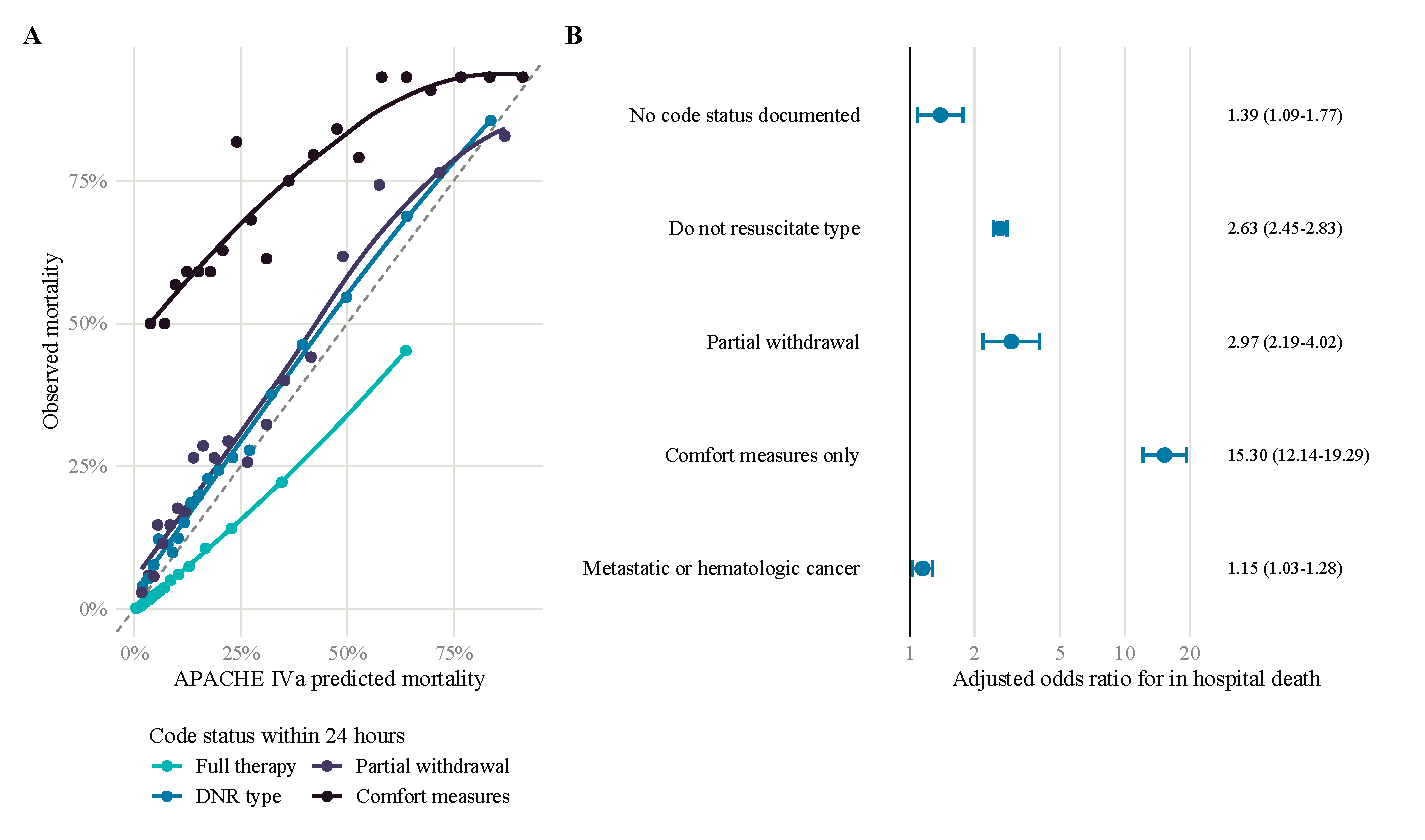
\includegraphics[width=\textwidth]{figures_pdf/Figure1_model_performance.pdf}
\caption{APACHE IVa performance by treatment limitation status.
(A) Calibration curves. Points are 5\% risk bins and the dashed line indicates
perfect calibration. (B) Adjusted odds ratios for in hospital death from a
logistic recalibration model, with full therapy as reference and standard errors
clustered on unit.}
\label{fig:performance}
\end{figure}

\begin{figure}[htbp]
\centering
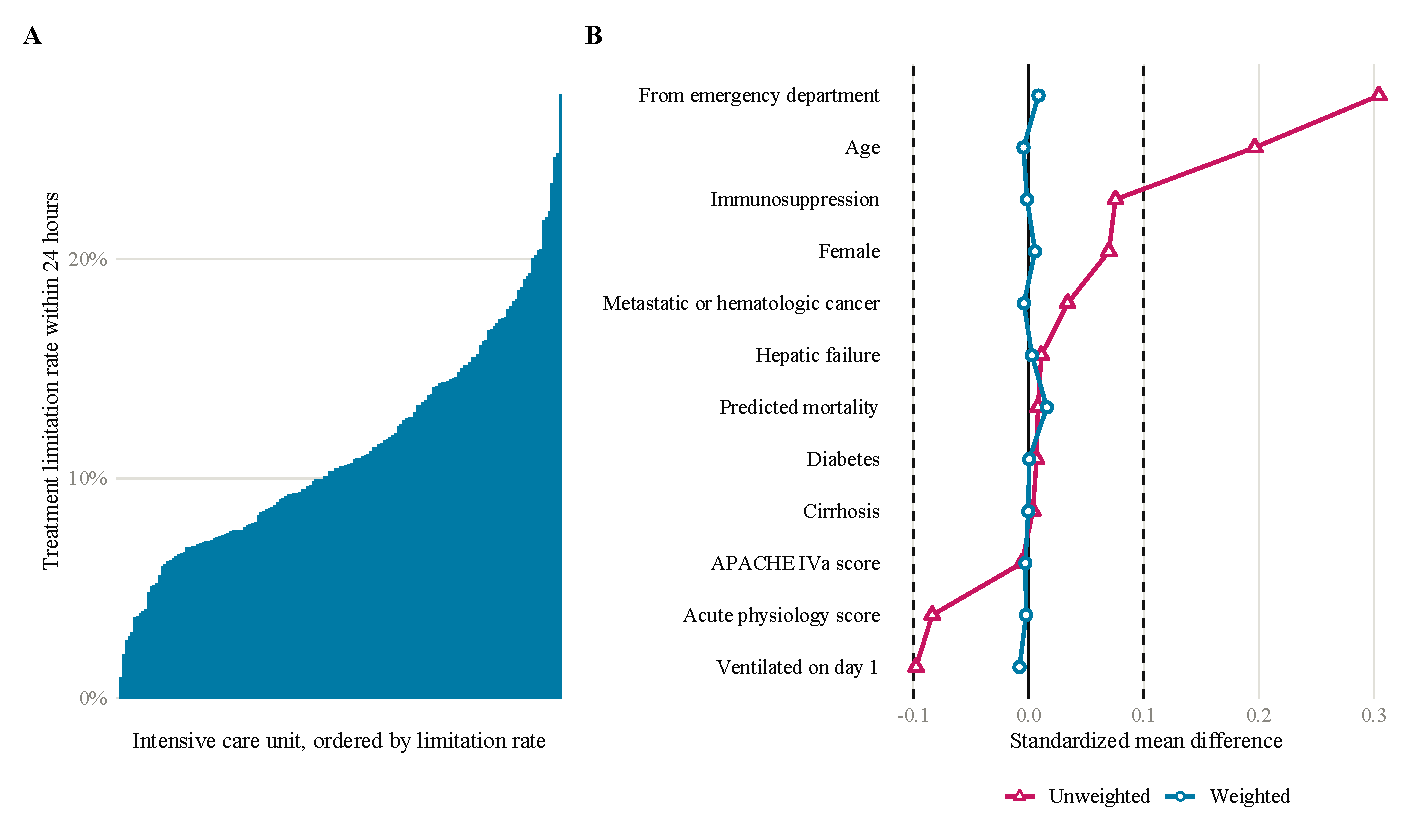
\includegraphics[width=\textwidth]{figures_pdf/Figure2_unit_variation.pdf}
\caption{Between unit variation in treatment limitation.
(A) Limitation rate within 24 hours across 162 units with 100 or more
admissions, ordered. (B) Standardized mean differences in patient
characteristics between units in the highest and lowest limitation quintile,
before and after inverse probability weighting. The shaded band marks the
conventional 0.1 threshold.}
\label{fig:variation}
\end{figure}

\begin{figure}[htbp]
\centering
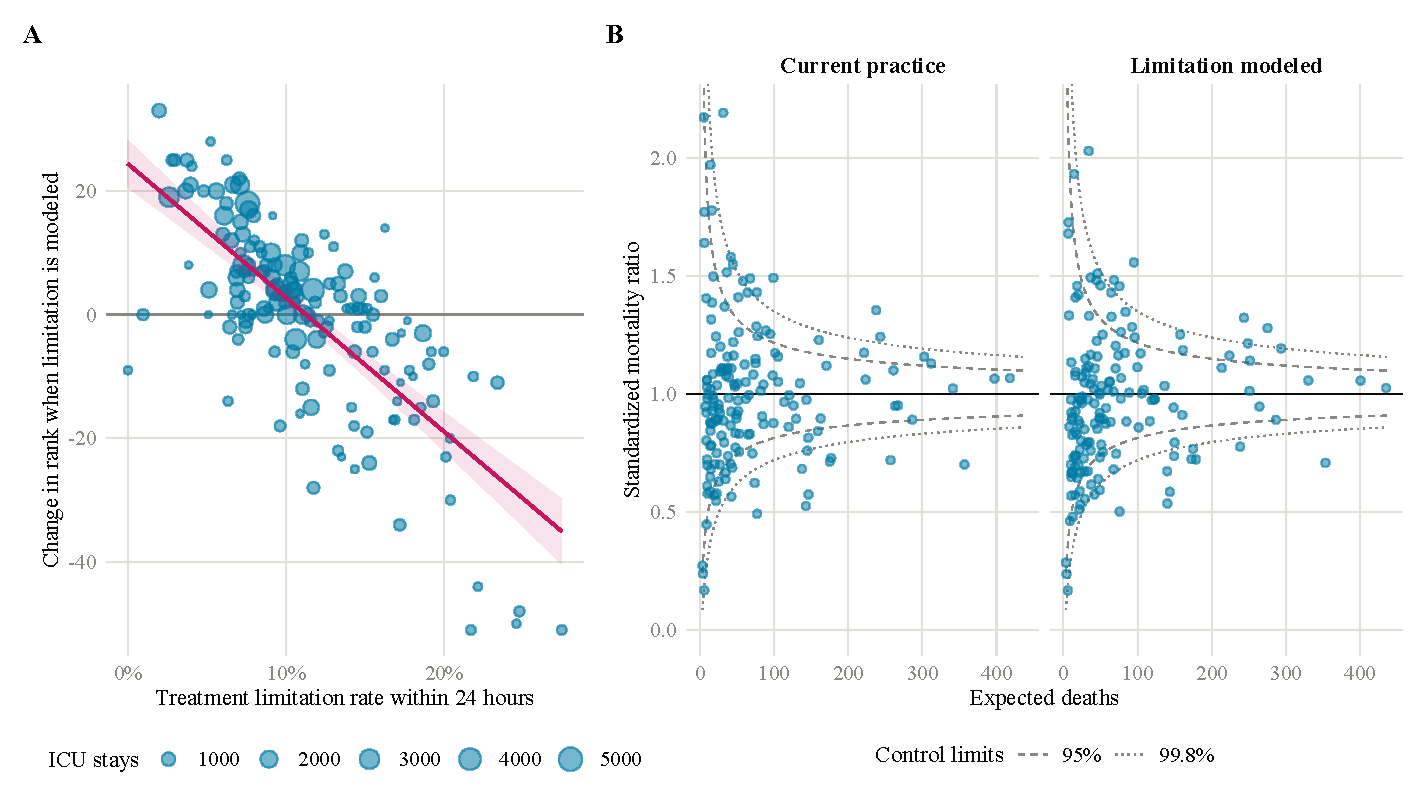
\includegraphics[width=\textwidth]{figures_pdf/Figure3_benchmarking.pdf}
\caption{Effect of modeling treatment limitation on unit benchmarking.
(A) Change in unit rank against limitation rate. Negative values indicate
improvement. (B) Funnel plots of standardized mortality ratio against expected
deaths under current practice and with limitation modeled, with 95\% and 99.8\%
exact Poisson control limits.}
\label{fig:benchmarking}
\end{figure}


\newpage
\bibliographystyle{unsrt}
\bibliography{references}

\end{document}
